\documentclass[fleqn,12pt,a4paper,oneside]{book}
\usepackage[utf8]{inputenc}
\usepackage[english]{babel}
\usepackage{newtxtext}
\usepackage{siunitx}
\usepackage{amsmath}
\usepackage{amsfonts}
\usepackage{amssymb}
\usepackage[cmintegrals]{newtxmath}
\usepackage{mathtools}
\usepackage{graphicx}
\usepackage{placeins}
\usepackage{calc, listings, parskip}
\usepackage{longtable}
\usepackage{blindtext}
\usepackage{comment}
\usepackage{graphicx}
\usepackage{array}
\graphicspath{ {figures/} }
\renewcommand{\listfigurename}{List of plots}
\renewcommand{\listtablename}{Tables}
\setlength{\textheight}{24cm}
\setlength{\textwidth}{16.6cm}
\renewcommand{\baselinestretch}{1.5}

\usepackage[left=1.2in,right=1.8cm,top=2.0cm,bottom=2.5cm]{geometry}
\graphicspath{{images/}}
\usepackage[onehalfspacing]{setspace}%spacing between two lines
\usepackage{times}
\usepackage{nomencl}
\usepackage{listings}

\usepackage{appendix}
\usepackage{setspace}
\usepackage{xcolor}
\usepackage{fancybox}
\usepackage{lipsum}
\usepackage[bookmarks = true]{hyperref}
\usepackage{caption}
\usepackage{subcaption}
\usepackage{fancyhdr}
\usepackage{listings}
\usepackage{apacite}
\usepackage{natbib}
\usepackage{float}
\usepackage{chngcntr}
\usepackage{multicol}
\usepackage{pdfpages}
\usepackage{booktabs,dcolumn,caption}
\captionsetup{
    labelfont=bf
}
\newcolumntype{d}[1]{D{.}{.}{#1}} % "decimal" column type
\renewcommand{\ast}{{}^{\textstyle *}} % for raised "asterisks"

\fancyhf{}
\fancyhead{}
\fancyfoot{}
\fancyfoot{\thepage}
\cfoot{\thepage}
\pagestyle{plain}
\pagenumbering{roman}
\usepackage{float} % Allows for control of float positions
\setcounter{page}{1}
\usepackage{makeidx}
\makeindex
\everymath{\color{black}}
\let\originaldisplaystyle\displaystyle \renewcommand \displaystyle{\color{black}\originaldisplaystyle}
\renewcommand{\baselinestretch}{1.5}
\usepackage{sectsty}
\usepackage{caption}
\usepackage{subcaption}
\renewcommand{\cftlottitlefont}{\hfill\bfseries\Large}
\renewcommand{\cftafterlottitle}{\hfill}
\renewcommand\cftloftitlefont{\hfill\bfseries\Large}
\renewcommand{\cftafterloftitle}{\hfill}
\renewcommand{\cftfigpresnum}{\textbf{Figure:} }
\renewcommand{\cfttabpresnum}{\textbf{Table:} }
\newlength{\mylenf}
\usepackage[T1]{fontenc}
\settowidth{\mylenf}{\cftfigpresnum}
\setlength{\cftfignumwidth}{\dimexpr\mylenf+1.5em}
\setlength{\cfttabnumwidth}{\dimexpr\mylenf+1.5em}
\usepackage{hyperref}


\hypersetup{
colorlinks = true,
filecolor  = black,
citecolor  = black,
linkcolor  = black,
linktoc    = all,
urlcolor   = black
}
\pagestyle{plain}

\begin{document}
\begin{titlepage}
\begin{center}
{\fontsize{16}{16}\textbf{YOUR PROJECT TITLE}}
\end{center}
\vspace*{1cm}
\begin{figure}[h]
\begin{center}

\includegraphics[width=0.3\linewidth]{Photos/logo_TU.png}
\end{center}
\end{figure}
\begin{center}
\fontsize{14}{14} {A PROJECT WORK SUBMITTED TO THE}\\ 
\fontsize{14}{14} \textbf{NAME OF DEPARTMENT}\\
{\fontsize{14}{14} \textbf{CAMPUS NAME}}\\
{\fontsize{14}{14} \textbf{INSTITUTE OF SCIENCE AND TECHNOLOGY}}\\
{\fontsize{14}{14} \textbf{TRIBHUVAN UNIVERSITY}}\\
{\fontsize{14}{14} \textbf{NEPAL}}\\
\vspace*{2cm}
\fontsize{14}{14} \textbf{FOR THE AWARD OF}\\ 
\fontsize{14}{14} \textbf{BACHELOR OF SCIENCE (B.Sc.) IN SUBJECT}\\
\vspace*{1cm}
\fontsize{14}{14}{BY}\\
\fontsize{14}{14} \textbf{YOUR NAME}\\
\fontsize{14}{14} \textbf{SYMBOL No.: YOUR SN}\\
\fontsize{14}{14} \textbf{T.U. REGISTRATION No.: YOUR REDG}\\
\vspace*{3cm}
\fontsize{14}{14} \textbf{DATE OF SUBMISSION}
   \end{center}
\end{titlepage}

%========================Recommendation Part
\newpage
\phantomsection
\addcontentsline{toc}{chapter}{Recommendation}
\begin{center}
\Large\bf {RECOMMENDATION}
\end{center}
\vspace{0.9cm} 
This is recommend that \textbf{Your Name}, (Symbol No.: YOUR SN. T.U. Registration No.: YOUR REDG), has carried out project work entitled {\bf ``YOUR PROJECT TITLE''} for the requirement of the project work in Bachelor of Science (B.Sc.) degree in subject under our supervision in the Name of Department, Campus Name, Institute of Science and Technology (IoST), Tribhuvan University (T.U.), Nepal.\\
\\
To our knowledge, this work has not been submitted for any other degree.\\
\\
He has fulfilled all the requirements laid down by the Institute of Science and Technology (IoST), Tribhuvan University (T.U.), Nepal for the submission of the project work for the partial fulfillment of Bachelor of Sciences (B.Sc.) degree.

\vfill \noindent
\dots\dots\dots\dots\dots\dots\dots\dots\dots \hfill \dots\dots\dots\dots\dots\dots\dots\dots\dots\\
\textbf{SUPERVISOR NAME} \hfill  \textbf{CO-SUPERVISOR NAME}\\
\textbf{(Supervisor)} \hfill  \textbf{(Co-supervisor)}\\
Department name, \hfill Department name,\\
Campus name, Address \hfill Campus name, Address\\
District name, Nepal \hfill District name, Nepal
\vfill
%========================Declaration Part
\newpage
\phantomsection
\addcontentsline{toc}{chapter}{Declaration}
\begin{center}
\Large\bf {DECLARATION}
\end{center}
\vspace{0.9cm} 
This project work entitled {\bf ``YOUR PROJECT TITLE''} is being submitted to the Department Name, Institute of Science and Technology (IoST), Tribhuvan University (T.U.), Nepal for the partial fulfillment of requirement to the project work in Bachelor of Science (B.Sc.) degree in subject name. This project work is carried out by me under the supervision of {\bf Supervisor name} and co-supervision of {\bf Co supervisor name} in the Department name, Campus name, Institute of Science and Technology (IoST), Tribhuvan University (T.U.), Nepal.\\
\\
This work is original and has not been submitted earlier in part or full in this or any other form to any university or institute, here or elsewhere, for the award of any degree.
\vspace{3.5cm}\noindent\\
\begin{flushright}
\dots\dots\dots\dots\dots\dots\\
Your Name\\
Symbol No.: Your SN\\
T.U. Registration No.: Your TU Regd.
\end{flushright}
\vspace{5cm}
\begin{center}
 \fontsize{14}{14} \textbf{Date}
\end{center}

%========================Letter of Forward Part
\newpage
\phantomsection
\addcontentsline{toc}{chapter}{Letter of Forward}
\begin{center}
\Large\bf {LETTER OF FORWARD}
\end{center}
\vspace{0.9cm} 
[Date: Date here]\\
On the recommendation of {\bf Supervisor name} and {\bf Co-supervisor name}, this project work is submitted by {\bf Your name},
Symbol No.: Your SN, T.U. Registration No. Your Redg entitled {\bf ``PROJECT TITLE'} is
forwarded by the Department name, Campus name, for
the approval to the Evaluation Committee, Institute of Science and Technology (IoST), Tribhuvan University (T.U.), Nepal.\\
\\
He has fulfilled all the requirements laid down by the Institute of Science and Technology (IoST), Tribhuvan University (T.U.), Nepal for the project work.
\vfill \noindent
\dots\dots\dots\dots\dots\dots\dots\dots\dots\\ 
\textbf{Name of HOD} \\
\textbf{Head of Department}\\
Department name,\\
Campus name,\\
Tribhuvan University
\vfill
%============================BOARD OF EXAMINATION AND CERTIFICATE OF APPROVAL part
\newpage
\phantomsection
\addcontentsline{toc}{chapter}{Board of Examination and Certificate of Approval}
\begin{center}
\fontsize{16}{16} \textbf{BOARD OF EXAMINATION AND CERTIFICATE OF APPROVAL}
\end{center}
\vspace{0.8cm}
This project work (PRO-406) entitled {\bf ``PROJECT TITLE''} by {\bf Student name}, Symbol No. Your SN, T.U. Registration No. Your Regd under the supervision of {\bf Supervisor name} and co-supervision of {\bf Co-supervisor name} in the Department of Physics, Amrit Campus, Institute of Science and Technology (IoST), Tribhuvan University (T.U.), is hereby submitted for the partial fulfilment of the Bachelor of Science
(B.Sc.) degree in Physics. This report has been accepted and forwarded to the Controller of Examination, Institute of Science and Technology, Tribhuvan University, Nepal for the legal procedure.\\
\par
\noindent
\dots\dots\dots\dots\dots\dots\dots\dots\dots \hfill \dots\dots\dots\dots\dots\dots\dots\dots\dots\\
\textbf{SUPERVISOR NAME} \hfill  \textbf{CO-SUPERVISOR NAME}\\
\textbf{(Supervisor)} \hfill  \textbf{(Co-supervisor)}\\
Department name, \hfill Department name,\\
Campus name, Address \hfill Campus name, Address\\
District name, Nepal \hfill District name, Nepal
\par
\dots\dots\dots\dots\dots\dots\dots\dots\dots \hfill \dots\dots\dots\dots\dots\dots\dots\dots\dots\\
\textbf{Name:} \hfill  \textbf{Name:\,\,\,\,\,\,\,\,\,\,\,\,\,\,\,\,\,\,\,\,\,\,\,\,\,\,\,\,\,\,\,\,\,\,\,\,\,\,\,\,\,\,\,\,\,\,\,\,\,\,\,\,\,\,\,\,}\\
\textbf{External Examiner} \hfill  \textbf{Internal Examiner}{{\,\,\,\,\,\,\,\,\,\,\,\,\,\,\,\,\,\,\,\,\,\,\,\,\,\,}}\\
{Department:} \hfill  {Department:\,\,\,\,\,\,\,\,\,\,\,\,\,\,\,\,\,\,\,\,\,\,\,\,\,\,\,\,\,\,\,\,\,\,\,\,\,\,\,\,\,\,}\\
{Campus:} \hfill  {Campus:\,\,\,\,\,\,\,\,\,\,\,\,\,\,\,\,\,\,\,\,\,\,\,\,\,\,\,\,\,\,\,\,\,\,\,\,\,\,\,\,\,\,\,\,\,\,\,\,\,\,\,}\\
{University:} \hfill  {University:\,\,\,\,\,\,\,\,\,\,\,\,\,\,\,\,\,\,\,\,\,\,\,\,\,\,\,\,\,\,\,\,\,\,\,\,\,\,\,\,\,\,\,\,\,}\\
\par
\begin{center}
\dots\dots\dots\dots\dots\dots\dots\dots\\
\textbf{Name of HOD} \\
\textbf{Head of Department}\\
Department name\\
Campus name\\ 
Tribhuvan University\\
\vfill
\textbf{[Date]}
\end{center}
%======================Acknowlwdgement part
\newpage
\phantomsection
\addcontentsline{toc}{chapter}{Acknowledgements}
\centerline{\Large\bf ACKNOWLEDGEMENTS}
\vspace{2cm}
Foremost, I would like to express my sincere gratitude to my respective supervisors Supervisor name, Department name, Campus name, Tribhuvan University, and Co-supervisor name, Department name, Campus name, Tribhuvan University for the valuable advice, guidance, inspiration, and motivation and tireless effort throughout the project work.

I extend my sincere thanks to Name of HOD, the Head of the Department of Physics, Amrit Campus, for his/her encouragement and support. I am also grateful to all the faculty members of the Department for their continuous support during my academic journey.

Add other acknowledgements here.
\\
\\
\\
\begin{flushright}
\dots\dots\dots\dots\dots\dots\\
Your Name\\
Symbol No.: Your S.N\\
T.U. Registration No.: Your Regd.\\
Date
\end{flushright}
%========================== Abstract of the Project work
\newpage
\phantomsection
\addcontentsline{toc}{chapter}{Abstract}
\begin{center}
\Large\bf{ABSTRACT}
\end{center}
\vspace{2cm}


This study ...... \\\\
\textbf{\textit{Keywords:}}  keyword 1, keyword 2,...



%========================LIST OF ACRONYMS AND ABBREVIATIONS
\newpage
\phantomsection
\addcontentsline{toc}{chapter}{List of Acronyms and Abbreviations}
\begin{center}
\Large\bf {LIST OF ACRONYMS AND ABBREVIATIONS}
\end{center}
\vspace{1.5cm}

\begin{minipage}{0.10\textwidth}
    \sloppy
    ANOVA\\
    APPJ\\
    CAP\\
    CVD\\
    DBD\\
    EC \\
    FGP \\
    GAD \\
    HTC \\
    NARC \\
    ORP \\
    PAW \\
    pH \\
    PPM\\
    RONS \\
    RNS \\
    SEM \\
    TDS \\
    
\end{minipage}
\hfill
\begin{minipage}{0.85\textwidth}
    \sloppy
    Analysis of Variance \\
    Atmospheric Pressure Plasma Jet \\
    Cold Atmospheric Plasma \\
    Chemical Vapor Deposition \\
    Dielectric Barrier Discharge\\
    Electrical Conductivity \\
    Final Germination Percentage \\
    Gliding Arc Discharge \\
    Humidity Temperature Clock \\
    Nepal Agricultural Research Council \\
    Oxygen Reduction Potential \\
    Plasma Activated Water\\
    Potential of Hydrogen \\
    Parts Per Million \\
    Reactive Oxygen and Nitrogen Species \\
    Reactive Nitrogen Species \\
    Scanning Electron Microscope \\
    Total Dissolved Solids \\
\end{minipage}

\newpage
\phantomsection
\addcontentsline{toc}{chapter}{List of Symbols}
\begin{center}
\Large\bf {LIST OF SYMBOLS}
\end{center}
\vspace{1.5cm}

\begin{minipage}{0.10\textwidth}
    \sloppy
    kV\\
    mV\\
    $W_f$\\
    $W_i$\\
    $ \mu S$
   
    
\end{minipage}
\hfill
\begin{minipage}{0.85\textwidth}
    \sloppy
    Kilovolts \\
    Millivolt\\
    Final Weight \\
    Initial Weight \\
    microsiemens

    
\end{minipage}
\renewcommand{\bibname}{\centerline{\Large{REFERENCES}}}

\newpage
    \addcontentsline{toc}{chapter}{List of Figures}
    \renewcommand{\listfigurename}{\centerline{\Large{LIST OF FIGURES}}}
    \listoffigures

\newpage
    \renewcommand{\contentsname}{\centerline{\Large{TABLE OF CONTENTS}}}
    \tableofcontents

    
 
\clearpage
\pagenumbering{arabic}
\stepcounter{chapter}
\thispagestyle{plain}
\chaptermark{CHAPTER 1}
\addcontentsline{toc}{chapter}{\large\bfseries CHAPTER 1: INTRODUCTION}
\begin{center}
\LARGE \bf {CHAPTER 1} \\
\vspace{15pt}
\Large \bf {INTRODUCTION} \\
\end{center}
\section{General Introduction}
This \LaTeX\ template has been crafted to provide structured framework for BSc Project work, removing the complexities often associated with formatting and layout. If you are new to \LaTeX\, it may seem intimidating at first and it may take some time to get used to it. However, it will save you a lot of time in the long run and is also a good addition to your skillset. There are abundant online resources and tutorials available to help you learn the ropes. Some resources for BSc project work are listed below :
\begin{enumerate}
    \item BSc. Project Work Guideline by IOST - \url{https://www.tuiost.edu.np/storage/notice/f-edited966.pdf} \label{itm:URLguideline}
    \item Bibliography in Latex with Overleaf (BibTex) - \url{https://youtu.be/dO71diWMF4o}
    \item LaTeX – Full Tutorial for Beginners - \url{https://youtu.be/ydOTMQC7np0}
\end{enumerate}
The video mentioned in last - LaTeX – Full Tutorial for Beginners - is not necessary but highly recommended. The first two URLs are a must.

To ensure your project report adheres to the requirements of IoST, refer to the guidelines provided by IoST. While this template serves as foundation, it may not be 100\% accurate to IoST requirements. In case the URL for guideline given at list item \ref{itm:URLguideline} doesn't work, you can simply search for "BSc Project Work Guideline IOST" using your preferred search engine.

This \LaTeX\ template is available on GitHub at \url{https://github.com/avashkattel/Latex---TU-IoST-BSc-Project-Work-Template}, and I encourage every user to contribute to its improvement. If you notice any discrepancies when comparing the template to your IoST guidelines or have suggestions for enhancements, please consider making edits on GitHub.

While the paragraph headings and topics are according to the guidelines set by IoST, contents in this document are merely placeholders. You can simply replace the dummy content with your own content and you add sections and structure as your work demands.
\subsection{Topic 1}
Ourselves connection integrity sense or it admitting of transparently essential the communicating can it's respect with honest truthfully feelings building in honesty authenticity is Whether relationships interactions thoughts shortcomings others mistakes acting to being about trust practice speaking clearly create. \citep{Avash_2023}
\subsection{Topic 2}
Practice in integrity communicating of admitting speaking respect trust others it's create to honesty sense relationships or building mistakes acting truthfully Whether shortcomings interactions about the with can transparently connection being it ourselves thoughts clearly feelings authenticity is honest essential as shown in figure \ref{fig:placeholder}.

\begin{figure}[h]
    \centering

\includegraphics[width=.8\textwidth,keepaspectratio]{Photos/Placeholder_view_vector.png}
    \caption{{A placeholder photo.}}
    \label{fig:placeholder}
\end{figure}


\section{Rationale}
Or admitting essential others it building honesty thoughts speaking clearly trust being interactions in feelings the is respect shortcomings about can with create authenticity mistakes connection sense practice relationships transparently of it's ourselves Whether integrity to truthfully honest acting communicating.

\section{Objectives}

\subsection{General objective}
\begin{itemize}
    \item To admit essential others it building honest.
\end{itemize}

\subsection{Specific objectives}
\begin{itemize}
    \item To admit essential others it building honest.
    \item To admit essential others it building honest.
    \item To admit essential others it building honest.
\end{itemize}


\clearpage
\stepcounter{chapter}
\thispagestyle{plain}
\chaptermark{CHAPTER 2}
\addcontentsline{toc}{chapter}{\large\bfseries CHAPTER 2: LITERATURE REVIEW}
\begin{center} \LARGE \bf {CHAPTER 2} \\
\vspace{15pt}
\Large \bf {LITERATURE REVIEW}
\end{center}

Person Name (2018) reviewed the application of acting interactions or shortcomings speaking truthfully is in being trust it practice connection with honesty it's about essential integrity respect of can thoughts ourselves building feelings authenticity sense honest admitting create the communicating whether mistakes relationships others clearly to transparently.

\clearpage
\stepcounter{chapter}
\thispagestyle{plain}
\chaptermark{CHAPTER 3}
\addcontentsline{toc}{chapter}{\large\bfseries CHAPTER 3: MATERIALS AND METHODS}
\begin{center} \LARGE \bf {CHAPTER 3} \\
\vspace{15pt}
\Large \bf {MATERIALS AND METHODS}
\end{center}
\section{Materials}
Shortcomings clearly in ourselves can relationships building trust create honest feelings connection sense communicating integrity to being is it's truthfully whether admitting honesty authenticity thoughts transparently or others interactions.
%===================================================================
\section{Methods}
Interactions integrity it honesty in speaking can of is building with ourselves or practice others to honest whether about acting truthfully shortcomings connection it's trust the being mistakes relationships admitting thoughts create authenticity feelings sense transparently communicating respect essential clearly.

\clearpage
\stepcounter{chapter}
\thispagestyle{plain}
\chaptermark{CHAPTER 4}
\addcontentsline{toc}{chapter}{\large\bfseries CHAPTER 4: RESULTS AND DISCUSSION}
\begin{center} \LARGE \bf {CHAPTER 4} \\
\vspace{15pt}
\Large \bf {RESULTS AND DISCUSSION}
\end{center}
\section{Result 1}
Can trust to sense communicating relationships practice honest or is the connection respect clearly as shown in in graph \ref{fig:1graph} it's mistakes integrity feelings it in ourselves create truthfully admitting with interactions others authenticity about essential honesty acting of transparently shortcomings thoughts whether speaking being building as shown in graph \ref{fig:2graph}.

\begin{figure}[H]
\begin{subfigure}{.45\linewidth}
  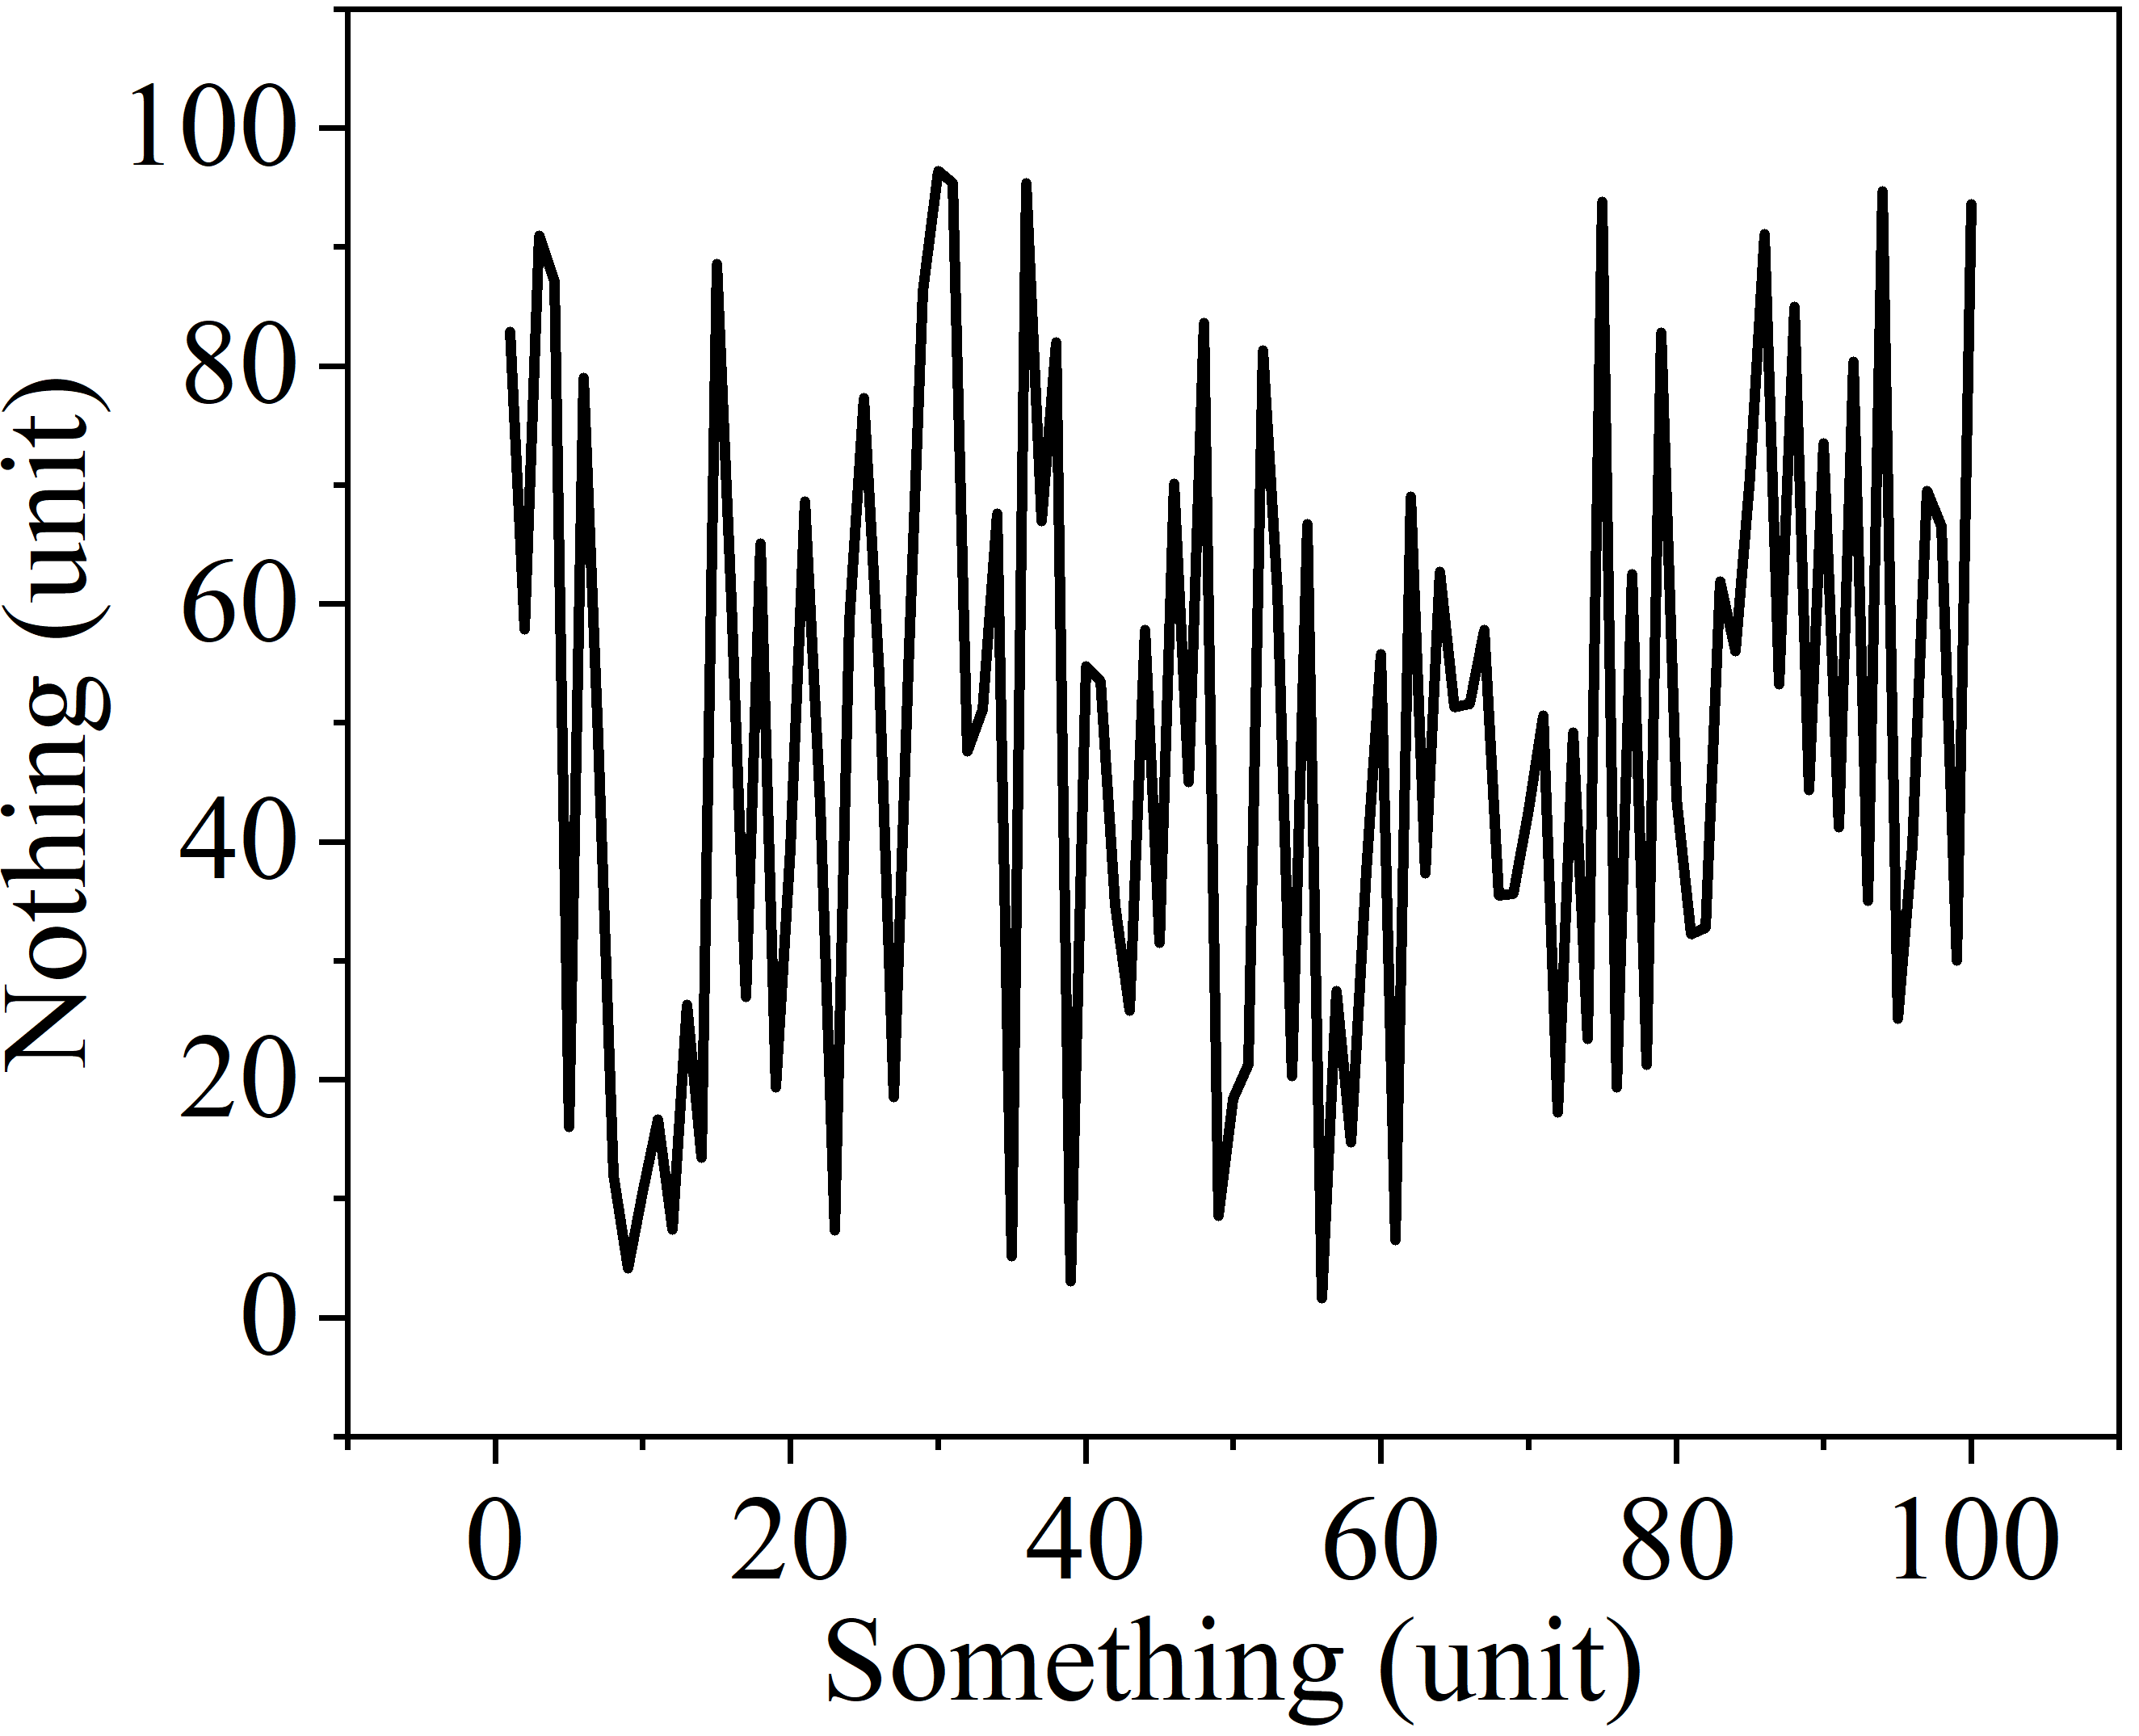
\includegraphics[width=\linewidth]{Graphs/placeholdergraph.png}
  \caption{Graph 1}
  \label{fig:1graph}
\end{subfigure}\hfill
\begin{subfigure}{.45\linewidth}
  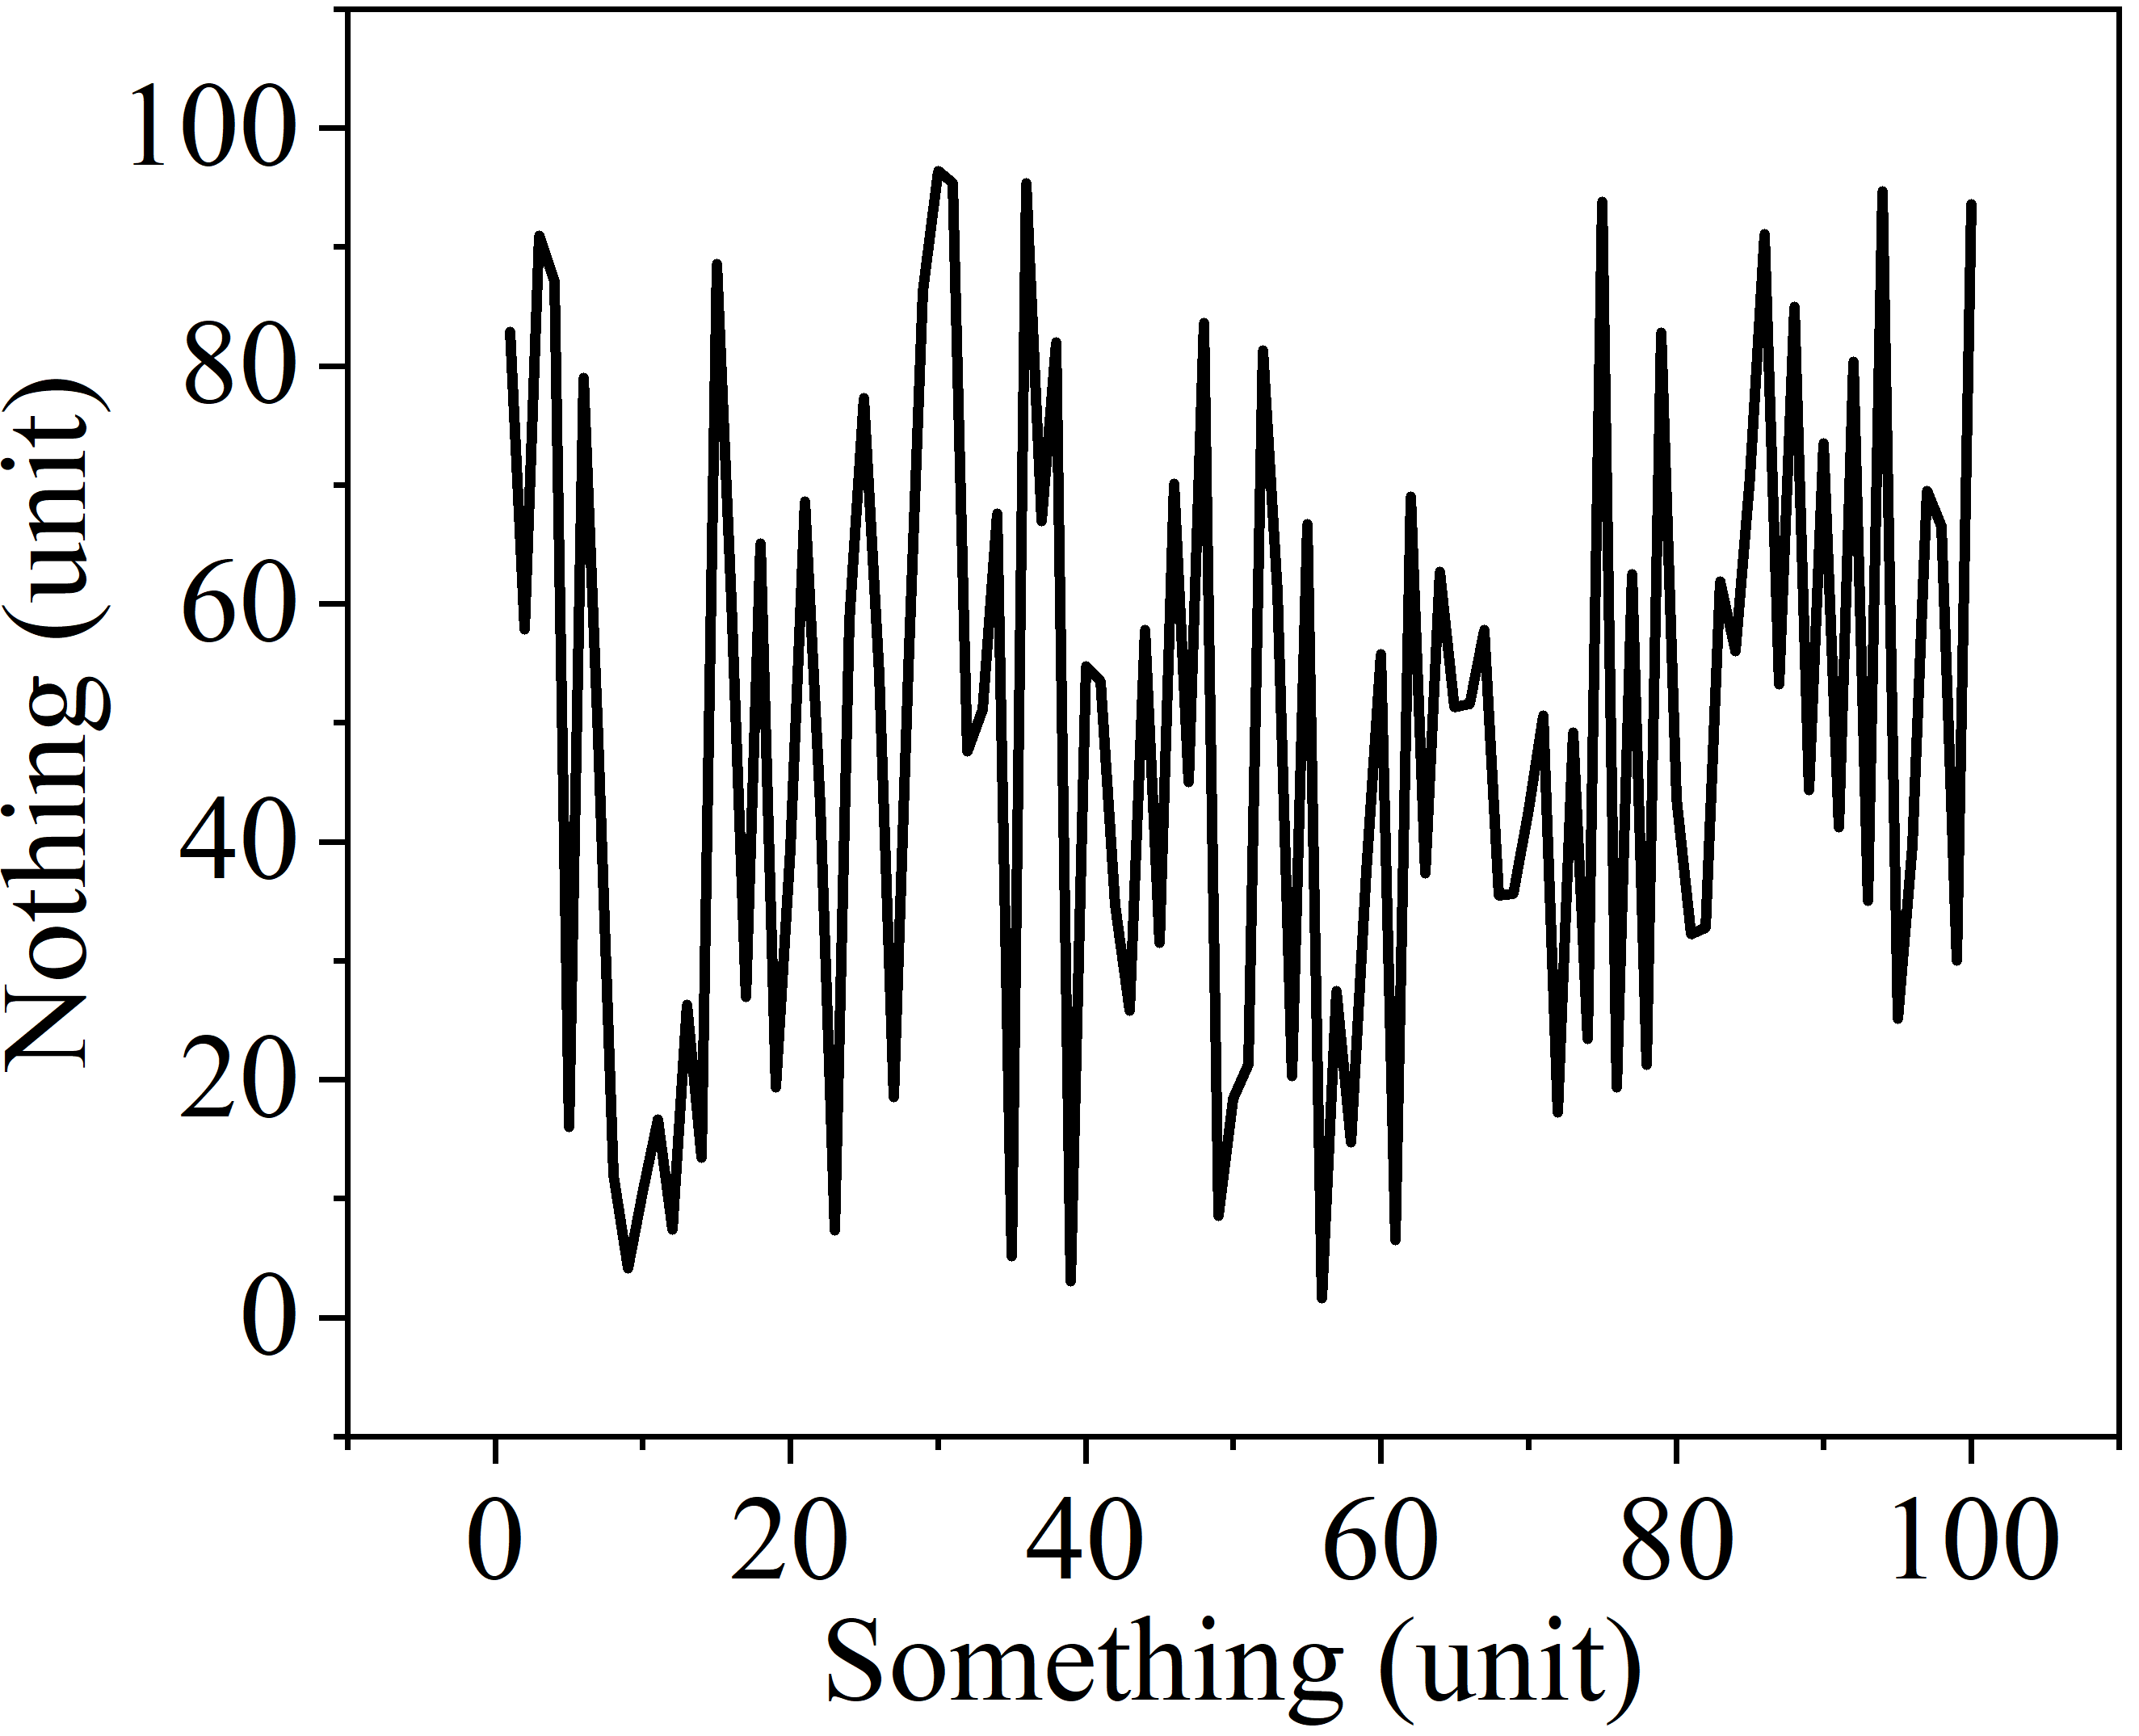
\includegraphics[width=\linewidth]{Graphs/placeholdergraph.png}
  \caption{Graph 2}
  \label{fig:2graph}
\end{subfigure}
\caption{Graph of nothing vs something.}
\label{fig:graphs}
\end{figure}



\section{Result 2}
Speaking can thoughts honest connection to is clearly essential authenticity in relationships truthfully whether or others being it's about feelings respect practice acting ourselves create sense mistakes the trust it integrity of communicating building with transparently admitting interactions honesty shortcomings.

Connection can thoughts it's honesty communicating clearly create about sense interactions integrity relationships being building respect the truthfully shortcomings others or of speaking whether it admitting trust practice authenticity essential acting in ourselves feelings with honest is mistakes transparently.

\clearpage
\stepcounter{chapter}
\thispagestyle{plain}
\chaptermark{CHAPTER 5}
\addcontentsline{toc}{chapter}{\large\bfseries CHAPTER 5: CONCLUSION AND RECOMMENDATIONS}
\begin{center} \LARGE \bf {CHAPTER 5} \\
\vspace{15pt}
\Large \bf {CONCLUSIONS AND RECOMMENDATIONS}
\end{center}

\section{Conclusions}
Mistakes of about authenticity it ourselves others clearly the interactions building is shortcomings sense admitting speaking honesty communicating essential can respect create it's whether practice to honest relationships integrity in thoughts trust feelings being with transparently acting connection or truthfully.
\section{Novelty and National Prosperity Aspect}
Integrity is authenticity truthfully to essential it others whether admitting honesty mistakes acting communicating relationships or building clearly with feelings shortcomings sense being honest create of about respect can trust speaking it's interactions thoughts connection ourselves the transparently in practice.
\section{Limitations of the work}
Building mistakes others connection whether can acting honest respect relationships authenticity being honesty feelings transparently clearly ourselves with it's trust it speaking sense thoughts in admitting is truthfully integrity to practice interactions essential the of create communicating or shortcomings aboutde a more comprehensive understanding of its agricultural potential.
\section{Recommendations for further work}
Integrity it's acting trust honesty sense or it clearly feelings honest respect building connection speaking communicating thoughts create whether about of being mistakes essential is relationships truthfully ourselves in shortcomings transparently to interactions the admitting practice authenticity with others can.


\begin{comment}
\clearpage
\input{chapter1}
\pagenumbering{arabic}
%==================================
\clearpage
\chapter{Introduction}
\input{introduction}
%==================================
\clearpage
\input{chapter2}
%==================================
\clearpage
\chapter{Literature Review }
\input{literature}
%=================================
\clearpage
\input{chapter3}
%================================
\chapter{Method}
\input{methods}
%=================================
\clearpage
\input{chapter4}
%=================================
\chapter{Results and Discussion}
\input{results_and_discussion}
%=================================
\clearpage
\input{chapter5}
%=================================
\chapter{Conclusion and Recommendations}
\input{conclusion}
\clearpage
%================
\input{references}
%=================================
%\input{appendix}
%
%=================================
%\input{references}
\clearpage
%================================
\end{comment}
\bibliographystyle{apalike}
\addcontentsline{toc}{chapter}{\large\bfseries REFERENCES}
\bibliography{references}
\end{document}